\documentclass[10pt]{article}

\usepackage[letterpaper,margin=1in]{geometry}
\usepackage[sfdefault]{plex-sans}
\usepackage{microtype}
\usepackage{parskip}
\usepackage{booktabs}
\usepackage{tabularx}
\usepackage{float}
\usepackage{xcolor}
\usepackage{enumitem}
\usepackage{tikz}
\usetikzlibrary{arrows.meta,positioning,fit,patterns,calc}
\usepackage{pgfplots}
\pgfplotsset{compat=1.18,every axis/.append style={font=\small},/pgf/number format/assume math mode=true}
\usepackage{needspace}
\usepackage[hidelinks]{hyperref}
\usepackage[numbers]{natbib}
\usepackage{caption}
\usepackage{titlesec}

% Captions under tables and figures, label in bold
\captionsetup{font=small,labelfont=bf,skip=6pt}
\titleformat{\section}{\Large\bfseries}{\thesection}{1em}{}
\titlespacing*{\section}{0pt}{1.6em}{0.6em}
\setlist{nosep,leftmargin=1.6em,topsep=2pt}
\renewcommand{\arraystretch}{1.25}
\newcolumntype{L}{>{\raggedright\arraybackslash}X}

\definecolor{caught}{HTML}{2A78D6}
\definecolor{missed}{HTML}{EB6834}

\begin{document}

\begin{center}
  {\LARGE\bfseries Can You Automate Expense Tracking in Singapore?\par}
  \vspace{6pt}
  {\large A free tracker built from bank alerts and statements, instead of typing in every payment\par}
  \vspace{4pt}
  {\small First version, November 2026\par}
  \vspace{14pt}
  {\large Madrid Lim\par}
  \vspace{2pt}
  {\small \texttt{github.com/StarlightsJourney/ugotmonee}\par}
\end{center}

\vspace{6pt}
\begin{center}\textbf{Abstract}\end{center}
\vspace{-6pt}
\begin{quote}
Most expense trackers in Singapore are manual, because banks don't give apps an open way to read personal transactions. But banks do send an email for some payments and a statement each month. I built ugotmonee, a free tracker that uses only those two, inside the user's own Google Sheet. It works, with one catch. Over five months of one person's accounts, the emails showed 51\% of the money spent but only 27\% of the payments. The rest, mostly small card and NETS QR payments, appeared only on the monthly statement. This report explains how to set the tracker up, why the emails miss so much, how the two sources are combined, and the problems I hit along the way.
\end{quote}

\section{Motivation}

There are two usual ways to track spending. One is to connect an app to your bank. In Singapore that is limited, as the next section shows. The other is to type every payment in yourself, which few people keep up.

But your bank already sends you two records of your spending:
\begin{itemize}
  \item \textbf{Email alerts}, seconds after many payments.
  \item \textbf{A statement}, once a month, listing every payment.
\end{itemize}
ugotmonee reads both and puts every payment into a Google Sheet. It sorts them into categories, draws charts, estimates your balance, and lists your subscriptions. There is no app to install, no account to create, and your data stays in your own Google account.

\Needspace{22\baselineskip}
\section{What already exists}

Table~\ref{tab:others} lists what we found in November 2026, and what each is missing.

\begin{table}[H]
\centering\small
\begin{tabularx}{\linewidth}{@{}>{\raggedright\arraybackslash}p{3.6cm}L@{}}
\toprule
\textbf{Kind} & \textbf{What's missing} \\
\midrule
Your bank's own planner (DBS NAV Planner, OCBC Financial OneView) & Sees only that bank's accounts. \\
SGFinDex & Gives balances and holdings, not a list of payments. \\
Multi-bank apps (Dobin, MySprout, Spendee) & Ask for your bank login or a paid plan. Seedly shut down at the end of 2025. \\
Email-forwarding services (Graiden) & Your bank emails are read on someone else's servers. \\
Open-source projects~\cite{lanbau,legitaxes,gmailpaylah,openexpense} & Each covers part of it: PayLah! or DBS emails only, or exports done by hand. None also reads OCBC or checks against statements. \\
\bottomrule
\end{tabularx}
\caption{Existing ways to track spending in Singapore~\cite{sprout,seedly,traceipt,graiden}. Based on the products' own pages and reviews, which may change.}
\label{tab:others}
\end{table}

The closest is lanbau/spend-tracker~\cite{lanbau}, which also runs on Apps Script and Gmail but reads only PayLah!. None we found reads both OCBC and DBS/POSB, combines emails with statements, and keeps everything in the user's own Google account.

\section{Setting it up}

Table~\ref{tab:need} lists what you need.

\begin{table}[H]
\centering
\begin{tabularx}{\linewidth}{@{}>{\bfseries}p{3.4cm}L@{}}
\toprule
A Google account & Its Gmail must receive your bank's email alerts. Google Sheets is free with it. \\
Bank email alerts & Turned on in your bank's internet banking, under e-Alerts. Turn on every kind, and set card alerts to the lowest amount. \\
Your statements & The monthly PDFs from internet banking. OCBC and DBS/POSB are supported. \\
Gemini key & Optional. Only if you want AI to sort merchants the tracker doesn't recognise. Free from Google AI Studio. \\
\bottomrule
\end{tabularx}
\caption{What you need.}
\label{tab:need}
\end{table}

\Needspace{12\baselineskip}
Then:
\begin{enumerate}
  \item \textbf{Make a Google Sheet} and open \emph{Extensions $\rightarrow$ Apps Script}.
  \item \textbf{Copy in the three files} from the \emph{apps-script} folder on GitHub. The README shows exactly where each one goes.
  \item \textbf{Reload the Sheet and click \emph{ugotmonee $\rightarrow$ Set up}.} Allow access when Google asks. It says the app is unverified because you just made it yourself: click \emph{Advanced}, then \emph{Go to ugotmonee}.
  \item \textbf{Type your name} in the Settings tab, the way your bank writes it. Money you move between your own accounts then isn't counted as spending.
  \item \textbf{Import your statements} with \emph{ugotmonee $\rightarrow$ Import statement (PDF)}.
\end{enumerate}

That's it. New payments appear within five minutes. On the 8th of each month you get an email if last month's statement hasn't been imported yet.

If the menu doesn't appear, or a window says \emph{permission denied}, you are probably signed in to more than one Google account. Open the Sheet in a private window signed in to just one.

\section{How much do bank emails show?}

For May to September I had both the emails and the statements, so I could check which payments had sent an email. Figure~\ref{fig:coverage} shows the result for each month.

\begin{figure}[H]
\centering
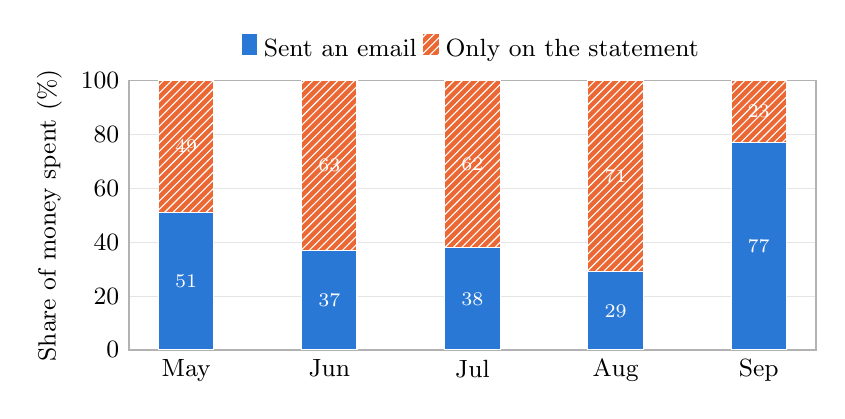
\begin{tikzpicture}
\begin{axis}[
  ybar stacked, bar width=20pt, width=0.85\linewidth, height=5cm,
  ymin=0, ymax=100, ylabel={Share of money spent (\%)},
  symbolic x coords={May,Jun,Jul,Aug,Sep}, xtick=data,
  legend style={at={(0.5,1.03)},anchor=south,legend columns=2,draw=none,font=\small},
  ymajorgrids, grid style={gray!20}, axis line style={gray!60}, tick style={draw=none},
  nodes near coords={\pgfmathprintnumber[fixed,precision=0]{\pgfplotspointmeta}},
  every node near coord/.append style={font=\scriptsize,color=white},
]
\addplot[fill=caught,draw=white] coordinates {(May,51) (Jun,37) (Jul,38) (Aug,29) (Sep,77)};
\addplot[fill=missed,draw=white,postaction={pattern=north east lines,pattern color=white}] coordinates {(May,49) (Jun,63) (Jul,62) (Aug,71) (Sep,23)};
\legend{Sent an email, Only on the statement}
\end{axis}
\end{tikzpicture}
\caption{Share of each month's spending that sent an email alert. September is higher only because one large card payment happened to send one.}
\label{fig:coverage}
\end{figure}

Overall, emails showed 51\% of the money but only 27\% of the payments. The missing ones were the small, frequent payments. Table~\ref{tab:missed} shows what they were.

\begin{table}[H]
\centering
\begin{tabularx}{\linewidth}{@{}lrrL@{}}
\toprule
\textbf{Kind of payment} & \textbf{Payments} & \textbf{Money} & \textbf{Why there was no email} \\
\midrule
Card & 235 & 71\% & Card alerts only go out above a minimum amount you choose. Bus and train fares are also charged in batches days later. \\
NETS QR & 120 & 27\% & Paid with the OCBC app, which offers no email alert for NETS QR. \\
Other & 3 & 2\% & Bank fees and a few transfers. \\
\bottomrule
\end{tabularx}
\caption{Payments that appeared only on the statement, May to September. ``Money'' is each kind's share of the missing amount.}
\label{tab:missed}
\end{table}

So a tracker that only reads emails makes every month look much cheaper than it was. Two habits fix most of it: turn on every kind of alert at the lowest amount, and import your statement each month.

\Needspace{16\baselineskip}
\section{How it works}

Figure~\ref{fig:flow} shows the parts. Everything runs inside your Google account, using Google Apps Script, Google's free tool for adding scripts to Sheets.

\begin{figure}[H]
\centering
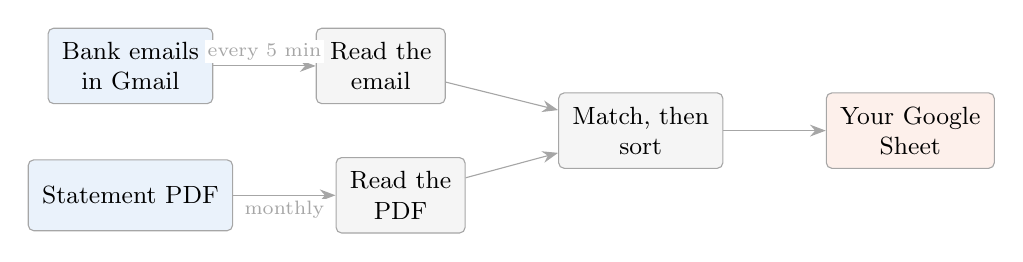
\begin{tikzpicture}[
  node distance=7mm and 13mm, font=\small,
  box/.style={draw=gray!70,rounded corners=2pt,align=center,inner sep=5pt,minimum height=9mm},
  src/.style={box,fill=caught!10}, proc/.style={box,fill=gray!8}, sink/.style={box,fill=missed!10},
  arr/.style={-{Stealth[length=2mm]},gray!70}]
\node[src] (gmail) {Bank emails\\in Gmail};
\node[src,below=of gmail] (pdf) {Statement PDF};
\node[proc,right=of gmail] (parse) {Read the\\email};
\node[proc,right=of pdf] (stmt) {Read the\\PDF};
\node[proc,right=13mm of $(parse.east)!0.5!(stmt.east)$,anchor=west] (rec) {Match, then\\sort};
\node[sink,right=of rec] (sheet) {Your Google\\Sheet};
\draw[arr] (gmail) -- node[above=1pt,font=\scriptsize,fill=white,inner sep=1pt]{every 5 min} (parse);
\draw[arr] (pdf) -- node[below=1pt,font=\scriptsize,fill=white,inner sep=1pt]{monthly} (stmt);
\draw[arr] (parse) -- (rec); \draw[arr] (stmt) -- (rec); \draw[arr] (rec) -- (sheet);
\end{tikzpicture}
\caption{How a payment gets into the Sheet. A payment seen in both an email and a statement becomes one row.}
\label{fig:flow}
\end{figure}

\textbf{Reading emails.} Every five minutes the script searches Gmail for emails from your banks and picks out the date, amount and who was paid. Any email that mentions money but isn't understood goes to an \emph{Unrecognised} tab, which is how new email formats get found.

\textbf{Reading statements.} The PDF is read inside your browser and never uploaded. Each import checks that the opening balance, minus money out, plus money in, equals the closing balance. If it doesn't, the import tells you something was missed.

\textbf{Matching the two.} Most payments appear twice: once in an email and once on the statement. They count as the same payment when the amount matches, the dates are within three days, and the names share a word. When in doubt the tracker keeps both, because a duplicate is easier to notice than a missing payment.

\textbf{Your balance.} The statement's closing balance is exact but only up to month end. After that, the tracker adds the emails since then. Because some payments send no email, you can also type in the balance your bank app shows, and it counts from there.

\textbf{Subscriptions.} The Recurring tab lists payments of about the same amount at a steady interval, like a phone plan, plus known services like streaming. If one stops appearing, it asks whether you cancelled it.

\textbf{Adding a payment by hand.} For a payment that sent no email, you type the date, what you bought and the amount into a new row. It counts straight away. When the statement arrives, a line with the same amount within three days is matched to your row instead of being added again.

\textbf{Categories.} Each payment gets a category from a built-in list of shops. Change a category once and the tracker remembers it for that shop. Optionally, Gemini sorts shops the list doesn't know. It sees only the shop's name, never amounts, dates or account numbers.

\Needspace{26\baselineskip}
\section{Problems I hit}

Table~\ref{tab:problems} lists the problems that took the most time to solve. Most aren't in Google's documentation.

\begin{table}[H]
\centering\footnotesize\renewcommand{\arraystretch}{1.12}
\begin{tabularx}{\linewidth}{@{}>{\raggedright\arraybackslash}p{2.8cm}LL@{}}
\toprule
\textbf{Problem} & \textbf{What happened} & \textbf{Fix} \\
\midrule
Reading the email & Every email failed to read & Gmail returns the email as raw bytes, not text as its documentation says. Accept both. \\
Too many emails at once & On the first run, Gmail's per-minute limit was hit & Stop when the limit is hit, and carry on from there five minutes later. \\
Six-minute limit & Google stops any script after six minutes & Read emails for three minutes, then save everything in one go. \\
New permissions & After an update, syncing quietly stopped & Click Set up again to approve the new permission. \\
Several Google accounts & ``Permission denied'' and a missing menu & A known Google bug. Use a private window with one account. \\
Wrong monthly totals & Every month showed the same total & One spreadsheet formula doesn't work across a list of months. Use a different one. \\
Silent failures & Scheduled runs failed without any message & The Settings tab now shows when the last sync ran and how it went. \\
Bank wording & ``FAST Payment / Receipt'' on a statement never matched its email & When the statement names nobody, match on amount, account and day. \\
\bottomrule
\end{tabularx}
\caption{The main problems, what happened, and the fix.}
\label{tab:problems}
\end{table}

\section{Privacy}

Your payments never leave your Google account, unless you turn on Gemini, which sees only shop names. The code is public, so it contains no real data. Test examples use made-up names and numbers, and the repository refuses any commit that contains a statement, a password or key, or an NRIC or phone number.

\section{What's next}

This is a first version. Right after this study I set card alerts to the lowest amount, so from November card payments should arrive by email within minutes instead of a month later. NETS QR depends on how you pay. With the OCBC app it can't be fixed: OCBC offers no email alert for it, so it waits for the statement. With DBS PayLah!, every payment sends an email, NETS QR included. So someone with only OCBC should pay by PayNow where the QR code allows; someone with DBS/POSB can scan with PayLah!. The next version of this report will measure how much that closes the gap.

\section{Limitations}

I tested one person's accounts at two banks. Other banks will send emails the tracker hasn't seen yet, and these will land in the Unrecognised tab. Payments your alert settings leave out only appear when you import the statement. E-wallet balances aren't tracked, which is fine as long as you keep the wallet empty.

\begin{thebibliography}{9}\small
\bibitem{sprout} MySprout. Expense tracker apps in Singapore: which banks sync? \url{https://mysprout.ai/blog/expense-tracker-apps-singapore-bank-sync}
\bibitem{seedly} Seedly. Best expense tracker apps in Singapore. \url{https://blog.seedly.sg/expense-tracker-apps/}
\bibitem{traceipt} Traceipt. What is SGFinDex? \url{https://traceipt.co/blog/what-is-sgfindex-singapore}
\bibitem{graiden} Graiden. Expense tracking in Singapore. \url{https://www.graiden.xyz/singapore}
\bibitem{lanbau} lanbau/spend-tracker. \url{https://github.com/lanbau/spend-tracker}
\bibitem{legitaxes} legitaxes/expense-tracker. \url{https://github.com/legitaxes/expense-tracker}
\bibitem{gmailpaylah} MarkHershey/gmail-paylah. \url{https://github.com/MarkHershey/gmail-paylah}
\bibitem{openexpense} pebblepaw/OpenExpense. \url{https://github.com/pebblepaw/OpenExpense}
\end{thebibliography}

\clearpage
\appendix

\section{Email formats}

These are the email formats the tracker reads. All examples are made up.

\begin{table}[H]
\centering\small
\begin{tabularx}{\linewidth}{@{}lLL@{}}
\toprule
\textbf{Bank} & \textbf{How to recognise it} & \textbf{Notes} \\
\midrule
OCBC & PayNow to a business: ``has been made to X using their Unique Entity Number'' & Times can look like ``16:51 PM''. \\
OCBC & PayNow to a person: ``using his/her Mobile'' & Names can contain extra spaces. \\
OCBC & PayNow failed: ``could not be made to'' & Skipped, since no money moved. \\
OCBC & Transfer to another bank: ``request to make the following transfer'' & Time written with a dot, ``11.14 AM''. \\
OCBC & NETS QR: ``The following NETS QR payment has been made'' & The account name leaves out ``OCBC''. \\
OCBC & ATM: ``was withdrawn from your account at an OCBC ATM'' & Sorted as cash. \\
OCBC & Card: ``was charged \ldots\ to your card'' & Only above your card alert amount. \\
OCBC & Red packet (e-Packet) & Sorted as gifts. \\
DBS & PayLah!: ``We refer to your PayLah! \ldots\ dated'' & No year given; worked out from when the email arrived. \\
DBS & Money received: ``You have received SGD \ldots\ via FAST transfer'' & Money coming in. OCBC sends no email for this. \\
\bottomrule
\end{tabularx}
\caption{Email formats from OCBC and DBS/POSB.}
\end{table}

\end{document}
